\PassOptionsToPackage{unicode=true}{hyperref} % options for packages loaded elsewhere
\PassOptionsToPackage{hyphens}{url}
%
\documentclass[10pt,xcolor=table,color={dvipsnames,usenames},ignorenonframetext,usepdftitle=false,french]{beamer}
\setbeamertemplate{caption}[numbered]
\setbeamertemplate{caption label separator}{: }
\setbeamercolor{caption name}{fg=normal text.fg}
\beamertemplatenavigationsymbolsempty
\usepackage{caption}
\captionsetup{skip=0pt,belowskip=0pt}
%\setlength\abovecaptionskip{-15pt}
\usepackage{lmodern}
\usepackage{amssymb,amsmath,mathtools,multirow}
\usepackage{float,hhline}
\usepackage{tikz}
\usepackage[tikz]{bclogo}
\usepackage{mathtools}
\usepackage{ifxetex,ifluatex}
\usepackage{fixltx2e} % provides \textsubscript
\ifnum 0\ifxetex 1\fi\ifluatex 1\fi=0 % if pdftex
  \usepackage[T1]{fontenc}
  \usepackage[utf8]{inputenc}
  \usepackage{textcomp} % provides euro and other symbols
\else % if luatex or xelatex
  \usepackage{unicode-math}
  \defaultfontfeatures{Ligatures=TeX,Scale=MatchLowercase}
\fi
\usetheme[coding=utf8,language=english,
,titlepagelogo=img/SACElogo.jpg
]{TorinoTh}
% use upquote if available, for straight quotes in verbatim environments
\IfFileExists{upquote.sty}{\usepackage{upquote}}{}
% use microtype if available
\IfFileExists{microtype.sty}{%
\usepackage[]{microtype}
\UseMicrotypeSet[protrusion]{basicmath} % disable protrusion for tt fonts
}{}
\IfFileExists{parskip.sty}{%
\usepackage{parskip}
}{% else
\setlength{\parindent}{0pt}
\setlength{\parskip}{6pt plus 2pt minus 1pt}
}
\usepackage{hyperref}
\hypersetup{
            pdftitle={Stability of Reg-ARIMA estimates: the case of leap year and outliers},
            pdfauthor={Dominique Ladiray et Alain Quartier-la-Tente},
            pdfborder={0 0 0},
            breaklinks=true}
\urlstyle{same}  % don't use monospace font for urls
\newif\ifbibliography
\usepackage{graphicx,grffile}
\makeatletter
\def\maxwidth{\ifdim\Gin@nat@width>\linewidth\linewidth\else\Gin@nat@width\fi}
\def\maxheight{\ifdim\Gin@nat@height>\textheight\textheight\else\Gin@nat@height\fi}
\makeatother
% Scale images if necessary, so that they will not overflow the page
% margins by default, and it is still possible to overwrite the defaults
% using explicit options in \includegraphics[width, height, ...]{}
\setkeys{Gin}{width=\maxwidth,height=\maxheight,keepaspectratio}
% Prevent slide breaks in the middle of a paragraph:
\widowpenalties 1 10000
\raggedbottom
\AtBeginPart{
  \let\insertpartnumber\relax
  \let\partname\relax
  \frame{\partpage}
}
\AtBeginSection{
  \ifbibliography
  \else
    \begin{frame}{Sommaire}
    \tableofcontents[currentsection, hideothersubsections]
    \end{frame}
  \fi
}
\setlength{\emergencystretch}{3em}  % prevent overfull lines
\providecommand{\tightlist}{%
  %\setlength{\itemsep}{0pt}
  \setlength{\parskip}{0pt}
  }
\setcounter{secnumdepth}{0}

% set default figure placement to htbp
\makeatletter
\def\fps@figure{htbp}
\makeatother

\usepackage{booktabs}
\usepackage{longtable}
\usepackage{array}
\usepackage{multirow}
\usepackage[table]{xcolor}
\usepackage{wrapfig}
\usepackage{float}
\usepackage{colortbl}
\usepackage{pdflscape}
\usepackage{tabu}
\usepackage{threeparttable}
\usepackage{threeparttablex}
\usepackage[normalem]{ulem}
\usepackage{makecell}

\title{Stability of Reg-ARIMA estimates: the case of leap year and outliers}
\ateneo{SACE Meeting \#5}
\author{Dominique Ladiray et Alain Quartier-la-Tente}
\date{}


\setrellabel{}

\setcandidatelabel{}

\rel{}
\division{Insee, Seasonal Adjustment Centre of Excellence (SACE)}

\departement{}
\makeatletter
\let\@@magyar@captionfix\relax
\makeatother

\DeclareMathOperator{\Cov}{Cov}
\newcommand{\E}[1]{\mathbb{E}\left[ #1 \right]}
\newcommand{\V}[1]{\mathbb{V}\left[ #1 \right]}
\newcommand{\cov}[2]{\Cov\left( #1\,,\,#2 \right)}

\begin{document}
\frame[plain,noframenumbering]{\titlepage}

\begin{frame}{Introduction to the seasonal adjustment procedure}

\centering
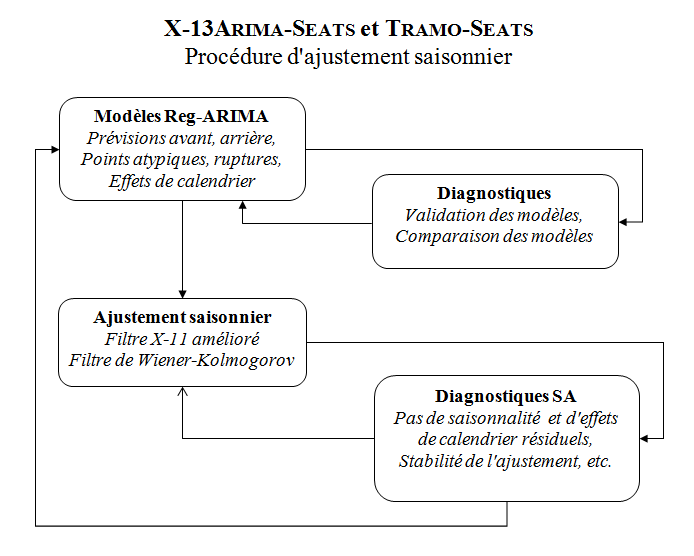
\includegraphics[height = 0.9\textheight]{img/MethodesX13-TS.png}

\end{frame}

\begin{frame}{Mathematical Writing of Reg-ARIMA}

Mathematical writing of the Reg-ARIMA Model in Seasonal Adjustment:

\[
 \begin{drcases}
\text{Additive: }& Y_t \\
\text{Multiplicative: }& \log(Y_t) 
\end{drcases} 
= \underbrace{\beta_0 LY_t + \beta_1 WD_t}_{\text{WD regressors}} + 
\underbrace{\sum_{i}\gamma_iO_{i,t}}_{\mathclap{\text{outliers}}} + \underbrace{\varepsilon_t}_{\sim ARIMA}
\]

\medskip

\pause
The goal of the study: illustrate some problems of instability of the
estimates with examples on:

\begin{itemize}
\item
  the leap year adjustment
\item
  the outliers estimates
\item
  the identification of the ARIMA model
\end{itemize}

\end{frame}

\section{The leap year adjustment}\label{the-leap-year-adjustment}

\subsection{How and when carry out the leap year
adjustment?}\label{how-and-when-carry-out-the-leap-year-adjustment}

\begin{frame}{Quand faut-il le corriger ?}

A leap year: one additional day in February \(\simeq\) every 4 years

\(\rightarrow\) takes into account the ``length of the month'' effect:
it is a calendar effect

\medskip

When to correct it \bcquestion 

\medskip \pause

According to the guidelines on seasonal adjustment, do so when:

\begin{itemize}
\item
  there is an economic sense to doing it
\item
  the effect is stable and statistically significant
\end{itemize}

\medskip \pause
Study of European IPI (1330 series): the leap year effect exists (but
not always measurable due to collection)

\end{frame}

\begin{frame}{To methods to proceed to the adjustment}

\begin{enumerate}
\item<1-> With the Reg-ARIMA model:
\[
LY_t = \begin{cases}
0.75 & \text{ in February during leap years} \\
-0.25  & \text{ in February during non leap years} \\
0 & \text{ for all other months}
\end{cases}
\]
\item<2-> Correcting values prior to modelling multiplying by a fixed proportion: 
\[\begin{cases}
\frac{28.25}{29} \simeq 0.974 & \text{ in February during leap years} \\
\frac{28.25}{28} \simeq 1.009 & \text{ in February during non leap years} \\
1 & \text{ for all other months}
\end{cases}
\]
\end{enumerate}

\pause[3]

\pause[4]

\(\rightarrow\) Study of estimates of the 1st method

\end{frame}

\subsection{Methodology of the study}\label{methodology-of-the-study}

\begin{frame}{Methodology used}

Methodology: \highlightbf{identified} the model throughout the entire
sample (ARIMA, outliers, etc.) and re-estimate month-by-month the past
values \highlightbf{setting} the first estimated date

\pause
\medskip
We considerded that the estimate has converged whe the estimated
coefficient remains:

\begin{itemize}
\item
  positive
\item
  not significantly different from last estimation
\item
  significant: stability of the choice to adjust the leap year effect
\end{itemize}

\(\implies\) European IPI: 410 converge

\end{frame}

\subsection{Examples}\label{examples}

\begin{frame}{Examples (1/2): IPI FR-0610 (extraction of crude
petroleum)}

\centering
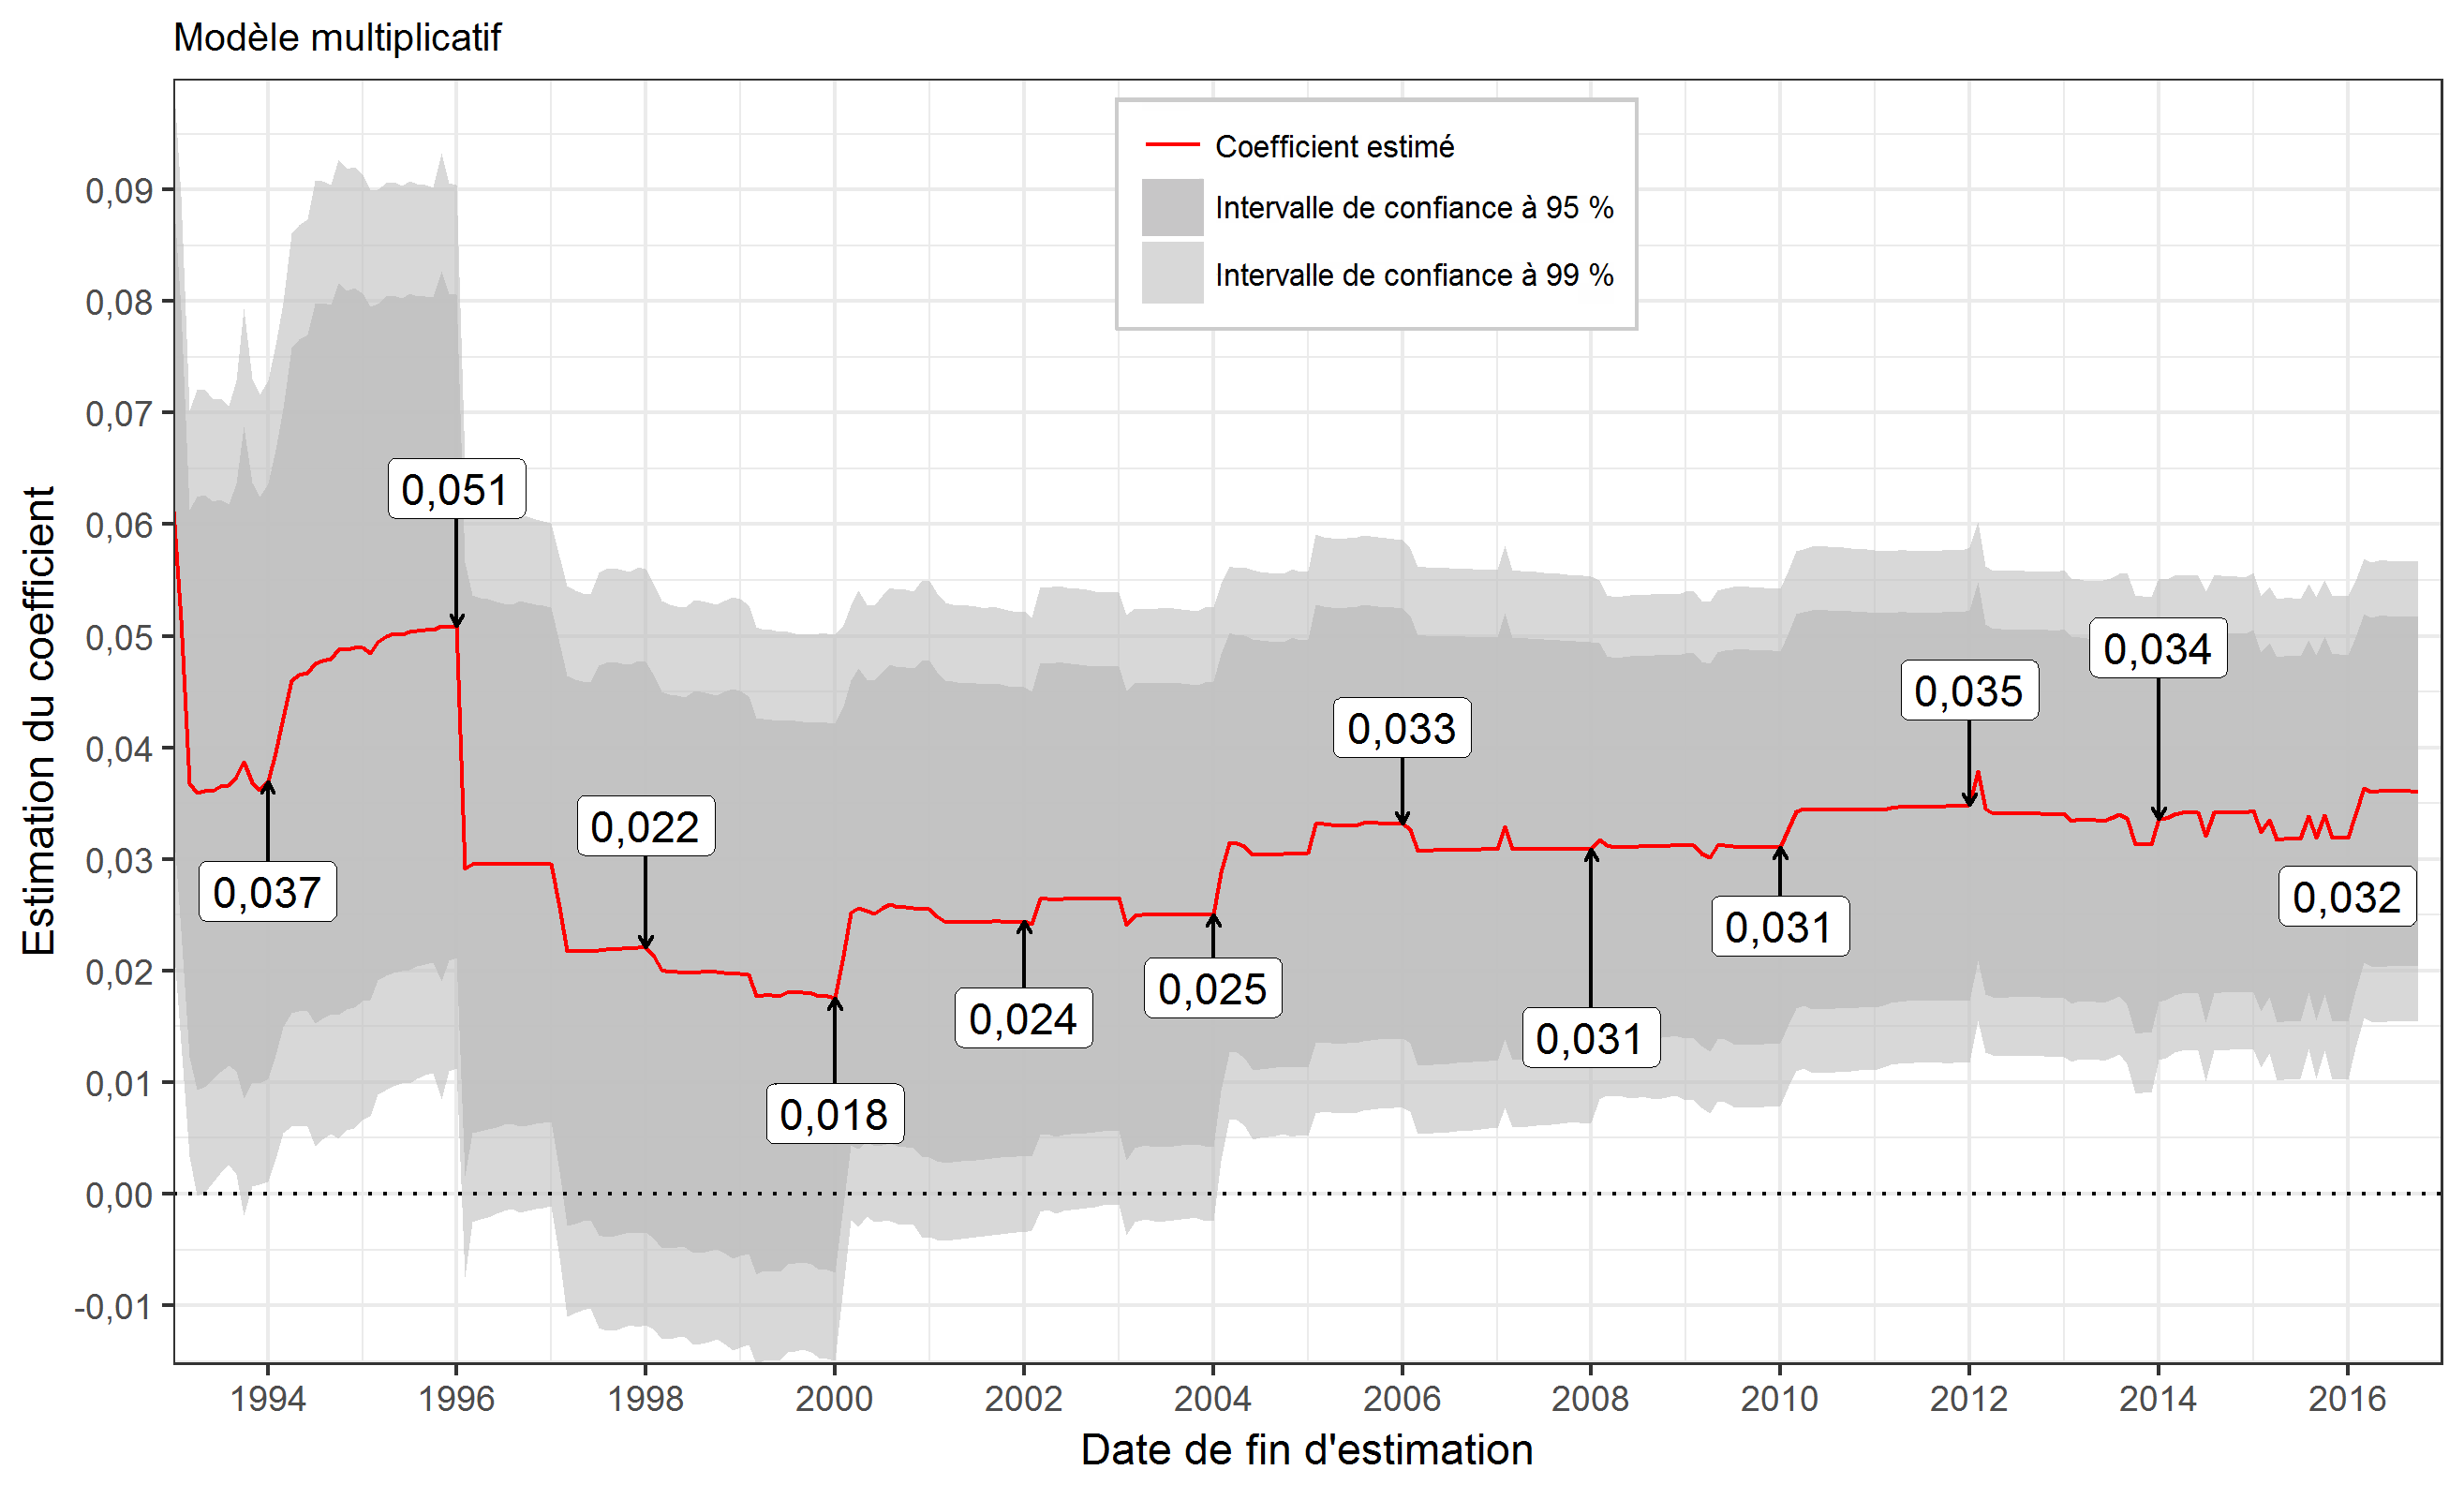
\includegraphics[width = \textwidth]{img/LYexemple1.png}

\end{frame}

\begin{frame}{Examples (2/2): IPI FR-1391 (manufacture of knitted and
crocheted fabrics)}

\centering
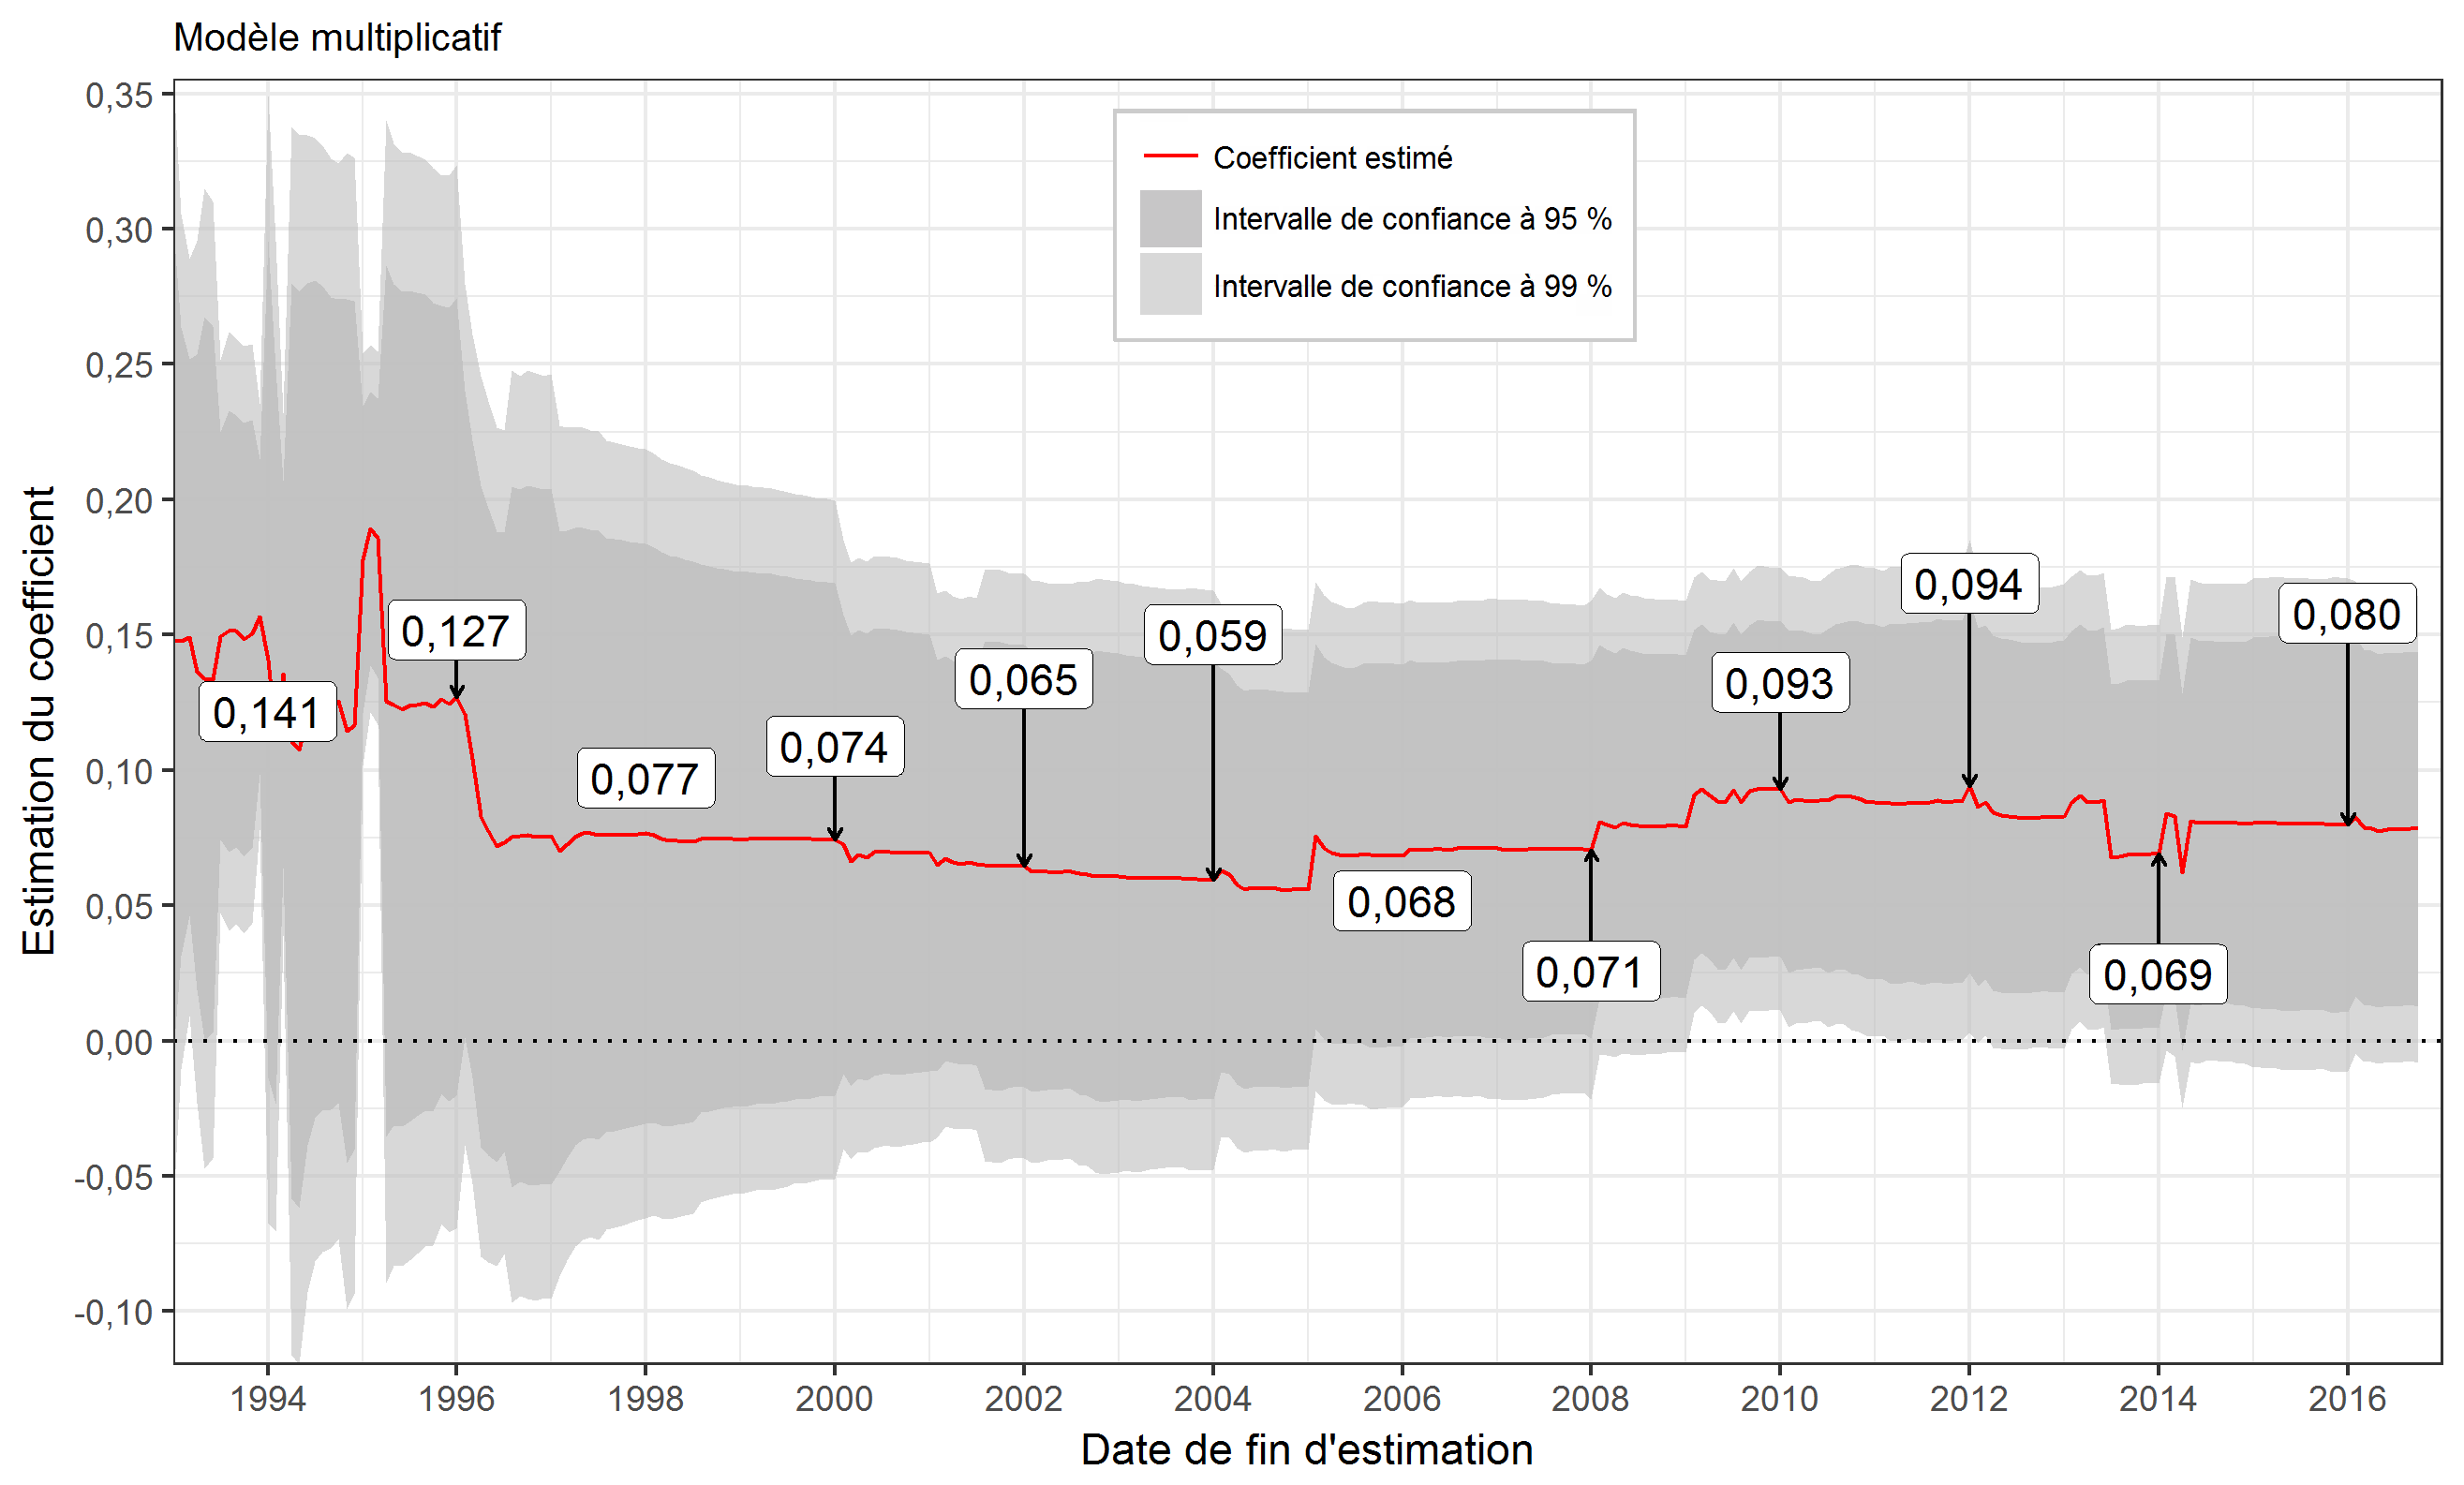
\includegraphics[width = \textwidth]{img/LYexemple2.png}

\end{frame}

\subsection{Results}\label{results}

\begin{frame}{A rather slow convergence\ldots{}}

\centering
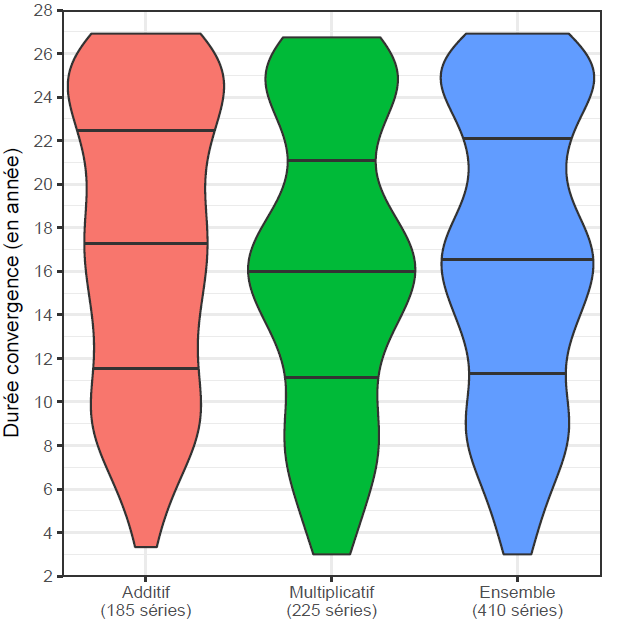
\includegraphics[height = 0.9\textheight]{img/LYconvergence.png}

\end{frame}

\begin{frame}{\ldots{} Towards a value not always coherent}

\centering
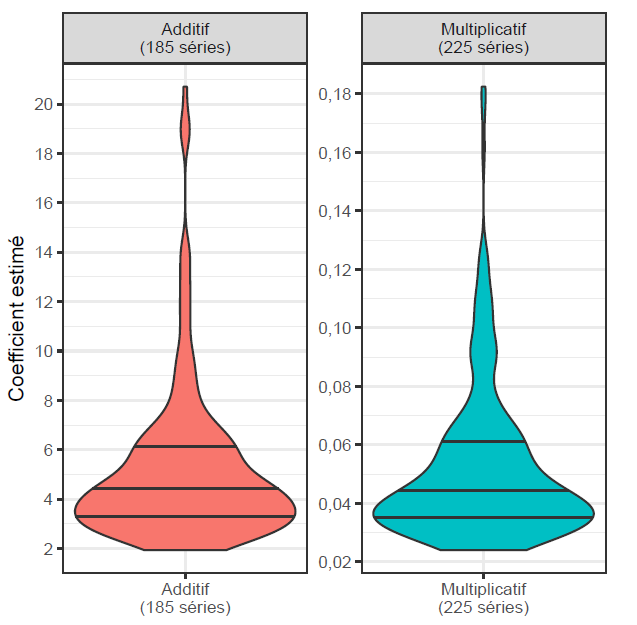
\includegraphics[height = 0.9\textheight]{img/LYvaleur.png}

\end{frame}

\begin{frame}{Comparison of the two correction methods}

\begin{figure}
\centering
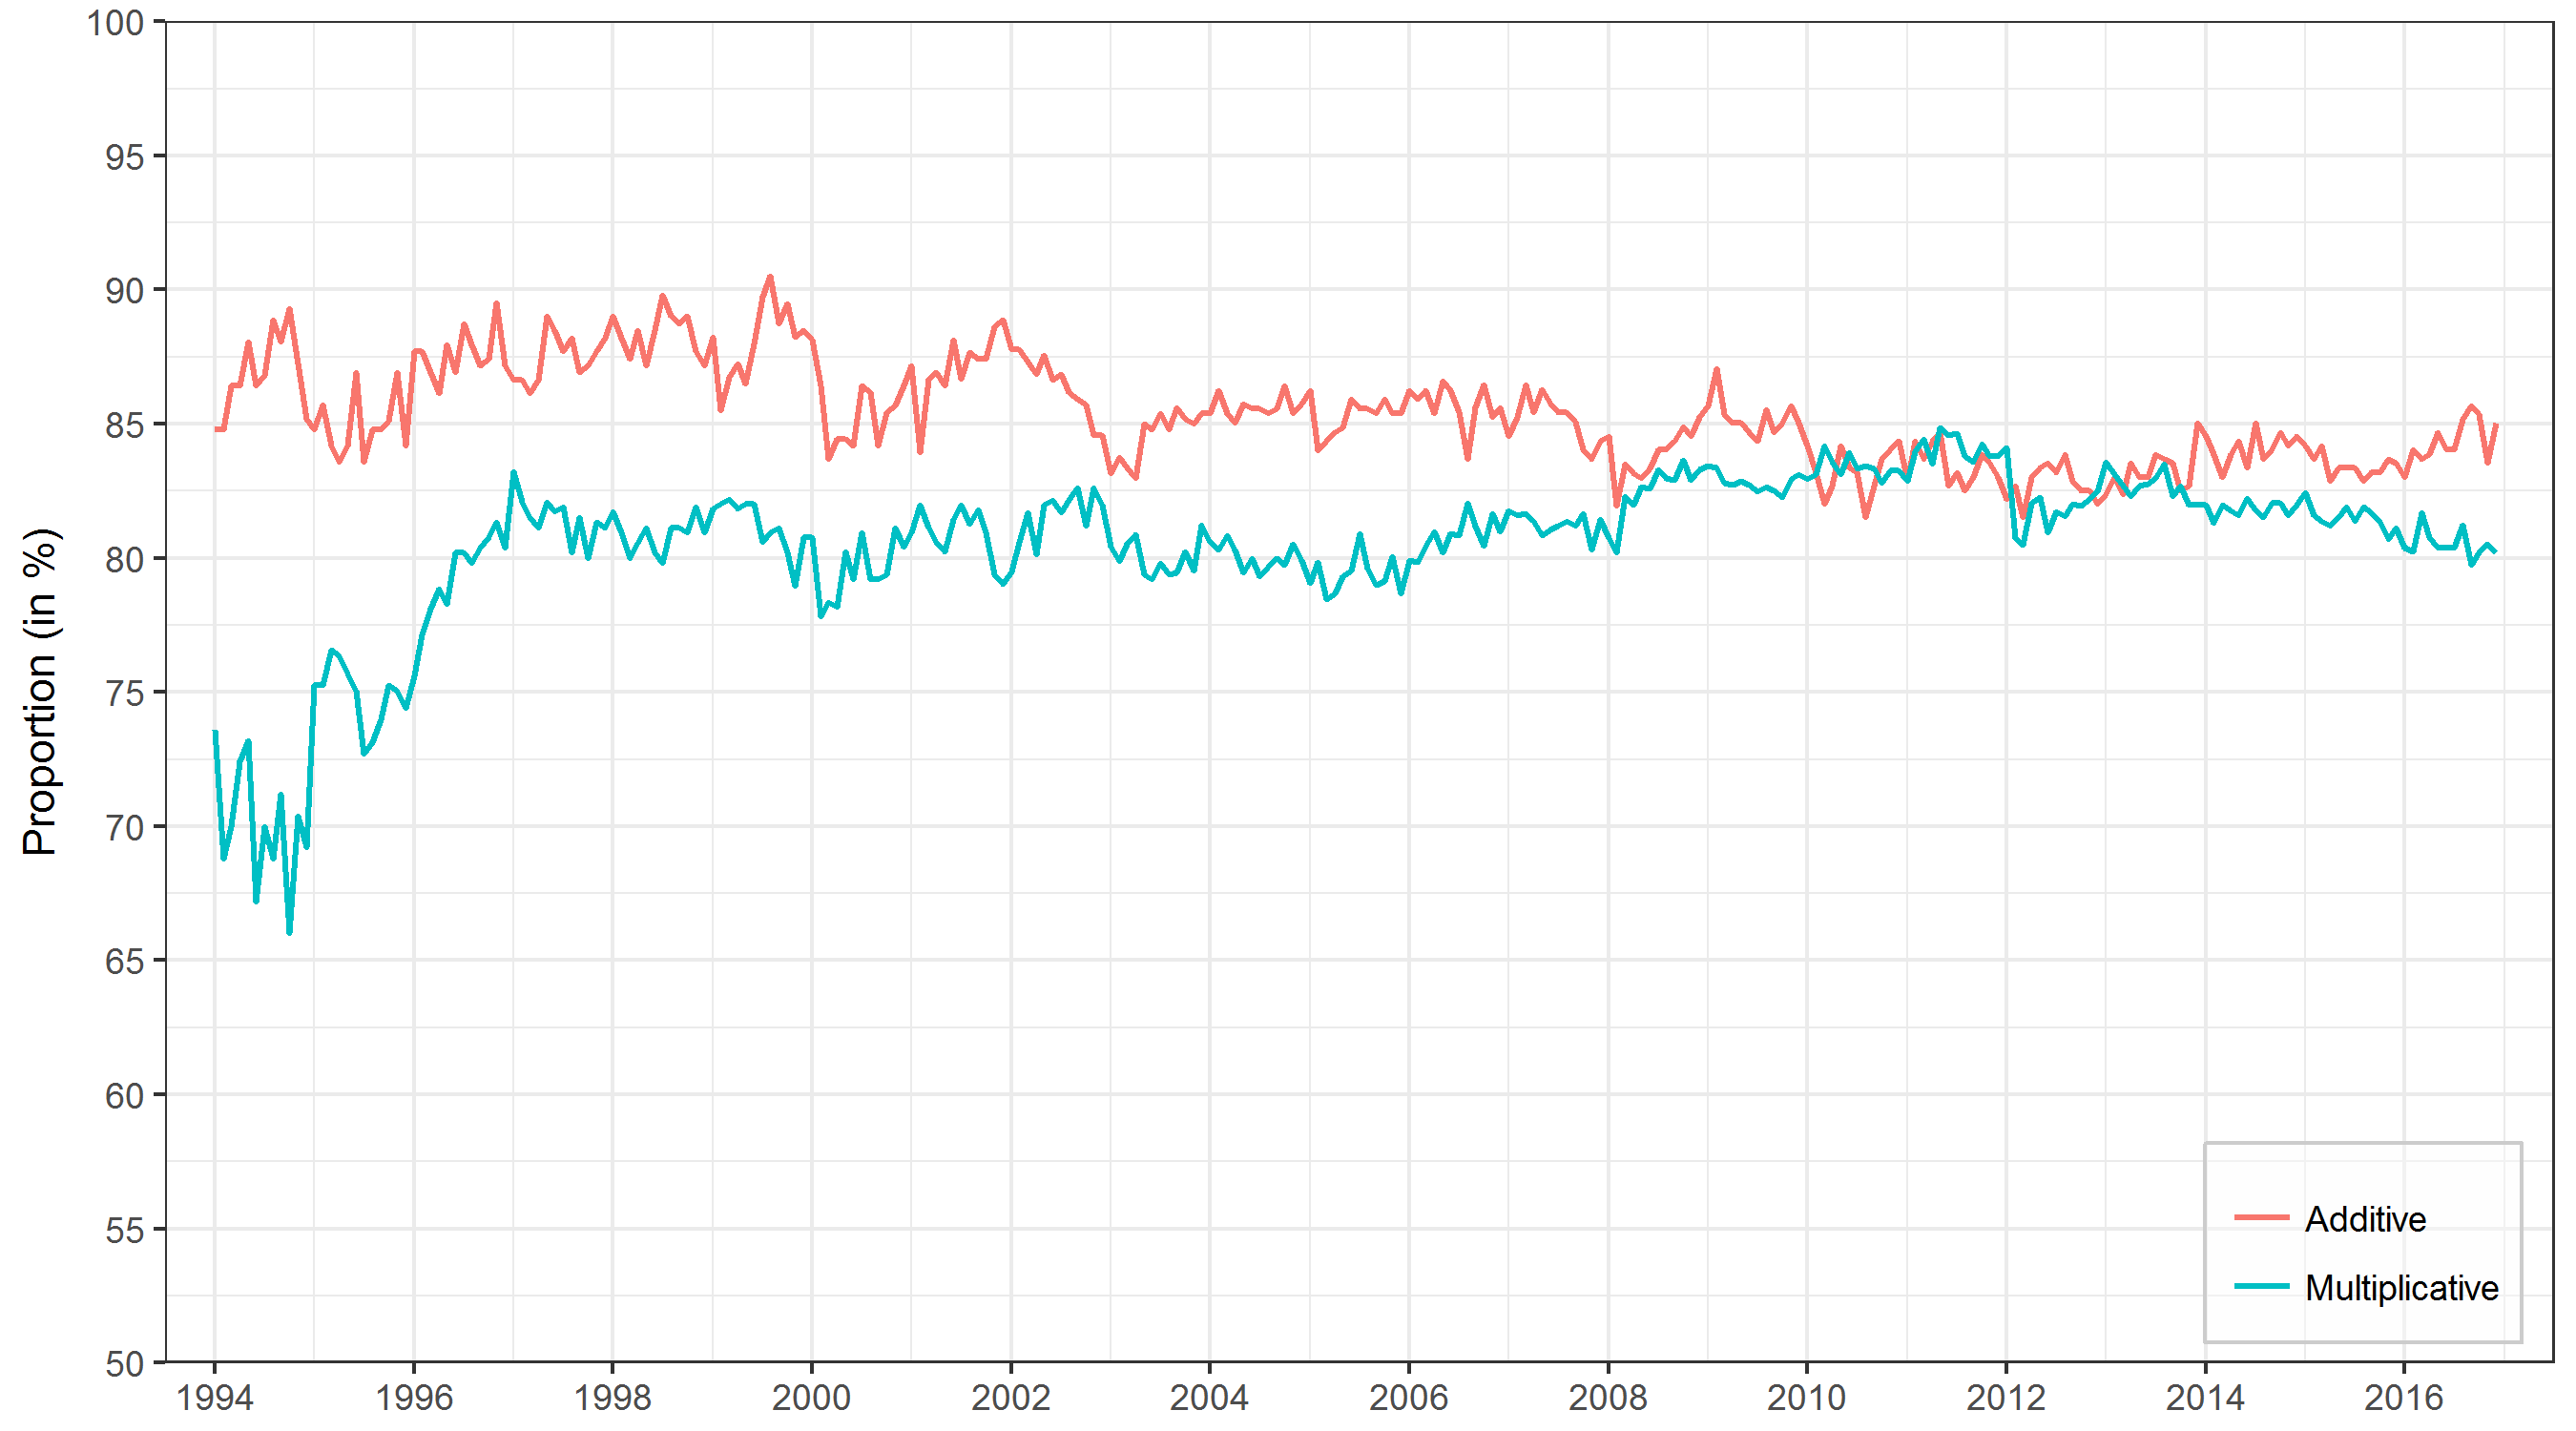
\includegraphics[width = \textwidth]{img/LYaicc.png}
\caption{
Percentage of series for which the AICC of the  2nd method (LY pre-adjustment) is lower than the AICC of the 1st method (LY regressor)}
\end{figure}

\end{frame}

\section{Outliers adjustment}\label{outliers-adjustment}

\subsection{Usuals outliers}\label{usuals-outliers}

\begin{frame}{Usuals outliers}

\smallskip

\begin{columns}
\begin{column}{0.6\textwidth}
\textbf{Additive outlier} (AO)
\end{column}
\begin{column}{0.3\textwidth}
% Created by tikzDevice version 0.10.1 on 2017-12-13 18:19:58
% !TEX encoding = UTF-8 Unicode
\begin{tikzpicture}[x=1pt,y=1pt]
\definecolor{fillColor}{RGB}{255,255,255}
\path[use as bounding box,fill=fillColor,fill opacity=0.00] (0,0) rectangle ( 93.95, 43.36);
\begin{scope}
\path[clip] (  0.00,  0.00) rectangle ( 93.95, 43.36);
\definecolor{drawColor}{RGB}{0,0,0}

\path[draw=drawColor,line width= 0.4pt,line join=round,line cap=round] (  3.48,  1.61) --
	(  4.40,  1.61) --
	(  5.31,  1.61) --
	(  6.23,  1.61) --
	(  7.14,  1.61) --
	(  8.06,  1.61) --
	(  8.97,  1.61) --
	(  9.89,  1.61) --
	( 10.81,  1.61) --
	( 11.72,  1.61) --
	( 12.64,  1.61) --
	( 13.55,  1.61) --
	( 14.47,  1.61) --
	( 15.38,  1.61) --
	( 16.30,  1.61) --
	( 17.22,  1.61) --
	( 18.13,  1.61) --
	( 19.05,  1.61) --
	( 19.96,  1.61) --
	( 20.88,  1.61) --
	( 21.79,  1.61) --
	( 22.71,  1.61) --
	( 23.63,  1.61) --
	( 24.54,  1.61) --
	( 25.46,  1.61) --
	( 26.37,  1.61) --
	( 27.29,  1.61) --
	( 28.20,  1.61) --
	( 29.12,  1.61) --
	( 30.04,  1.61) --
	( 30.95,  1.61) --
	( 31.87,  1.61) --
	( 32.78,  1.61) --
	( 33.70,  1.61) --
	( 34.61,  1.61) --
	( 35.53,  1.61) --
	( 36.44,  1.61) --
	( 37.36,  1.61) --
	( 38.28,  1.61) --
	( 39.19,  1.61) --
	( 40.11,  1.61) --
	( 41.02,  1.61) --
	( 41.94,  1.61) --
	( 42.85,  1.61) --
	( 43.77,  1.61) --
	( 44.69,  1.61) --
	( 45.60,  1.61) --
	( 46.52,  1.61) --
	( 47.43, 41.76) --
	( 48.35,  1.61) --
	( 49.26,  1.61) --
	( 50.18,  1.61) --
	( 51.10,  1.61) --
	( 52.01,  1.61) --
	( 52.93,  1.61) --
	( 53.84,  1.61) --
	( 54.76,  1.61) --
	( 55.67,  1.61) --
	( 56.59,  1.61) --
	( 57.51,  1.61) --
	( 58.42,  1.61) --
	( 59.34,  1.61) --
	( 60.25,  1.61) --
	( 61.17,  1.61) --
	( 62.08,  1.61) --
	( 63.00,  1.61) --
	( 63.92,  1.61) --
	( 64.83,  1.61) --
	( 65.75,  1.61) --
	( 66.66,  1.61) --
	( 67.58,  1.61) --
	( 68.49,  1.61) --
	( 69.41,  1.61) --
	( 70.33,  1.61) --
	( 71.24,  1.61) --
	( 72.16,  1.61) --
	( 73.07,  1.61) --
	( 73.99,  1.61) --
	( 74.90,  1.61) --
	( 75.82,  1.61) --
	( 76.74,  1.61) --
	( 77.65,  1.61) --
	( 78.57,  1.61) --
	( 79.48,  1.61) --
	( 80.40,  1.61) --
	( 81.31,  1.61) --
	( 82.23,  1.61) --
	( 83.15,  1.61) --
	( 84.06,  1.61) --
	( 84.98,  1.61) --
	( 85.89,  1.61) --
	( 86.81,  1.61) --
	( 87.72,  1.61) --
	( 88.64,  1.61) --
	( 89.56,  1.61) --
	( 90.47,  1.61);
\end{scope}
\end{tikzpicture}

\end{column}
\end{columns}

\begin{columns}
\begin{column}{0.6\textwidth}
\textbf{Level Shift} (LS)
\end{column}
\begin{column}{0.3\textwidth}
% Created by tikzDevice version 0.10.1 on 2017-12-13 18:19:58
% !TEX encoding = UTF-8 Unicode
\begin{tikzpicture}[x=1pt,y=1pt]
\definecolor{fillColor}{RGB}{255,255,255}
\path[use as bounding box,fill=fillColor,fill opacity=0.00] (0,0) rectangle ( 93.95, 43.36);
\begin{scope}
\path[clip] (  0.00,  0.00) rectangle ( 93.95, 43.36);
\definecolor{drawColor}{RGB}{0,0,0}

\path[draw=drawColor,line width= 0.4pt,line join=round,line cap=round] (  3.48,  1.61) --
	(  4.40,  1.61) --
	(  5.31,  1.61) --
	(  6.23,  1.61) --
	(  7.14,  1.61) --
	(  8.06,  1.61) --
	(  8.97,  1.61) --
	(  9.89,  1.61) --
	( 10.81,  1.61) --
	( 11.72,  1.61) --
	( 12.64,  1.61) --
	( 13.55,  1.61) --
	( 14.47,  1.61) --
	( 15.38,  1.61) --
	( 16.30,  1.61) --
	( 17.22,  1.61) --
	( 18.13,  1.61) --
	( 19.05,  1.61) --
	( 19.96,  1.61) --
	( 20.88,  1.61) --
	( 21.79,  1.61) --
	( 22.71,  1.61) --
	( 23.63,  1.61) --
	( 24.54,  1.61) --
	( 25.46,  1.61) --
	( 26.37,  1.61) --
	( 27.29,  1.61) --
	( 28.20,  1.61) --
	( 29.12,  1.61) --
	( 30.04,  1.61) --
	( 30.95,  1.61) --
	( 31.87,  1.61) --
	( 32.78,  1.61) --
	( 33.70,  1.61) --
	( 34.61,  1.61) --
	( 35.53,  1.61) --
	( 36.44,  1.61) --
	( 37.36,  1.61) --
	( 38.28,  1.61) --
	( 39.19,  1.61) --
	( 40.11,  1.61) --
	( 41.02,  1.61) --
	( 41.94,  1.61) --
	( 42.85,  1.61) --
	( 43.77,  1.61) --
	( 44.69,  1.61) --
	( 45.60,  1.61) --
	( 46.52,  1.61) --
	( 47.43, 41.76) --
	( 48.35, 41.76) --
	( 49.26, 41.76) --
	( 50.18, 41.76) --
	( 51.10, 41.76) --
	( 52.01, 41.76) --
	( 52.93, 41.76) --
	( 53.84, 41.76) --
	( 54.76, 41.76) --
	( 55.67, 41.76) --
	( 56.59, 41.76) --
	( 57.51, 41.76) --
	( 58.42, 41.76) --
	( 59.34, 41.76) --
	( 60.25, 41.76) --
	( 61.17, 41.76) --
	( 62.08, 41.76) --
	( 63.00, 41.76) --
	( 63.92, 41.76) --
	( 64.83, 41.76) --
	( 65.75, 41.76) --
	( 66.66, 41.76) --
	( 67.58, 41.76) --
	( 68.49, 41.76) --
	( 69.41, 41.76) --
	( 70.33, 41.76) --
	( 71.24, 41.76) --
	( 72.16, 41.76) --
	( 73.07, 41.76) --
	( 73.99, 41.76) --
	( 74.90, 41.76) --
	( 75.82, 41.76) --
	( 76.74, 41.76) --
	( 77.65, 41.76) --
	( 78.57, 41.76) --
	( 79.48, 41.76) --
	( 80.40, 41.76) --
	( 81.31, 41.76) --
	( 82.23, 41.76) --
	( 83.15, 41.76) --
	( 84.06, 41.76) --
	( 84.98, 41.76) --
	( 85.89, 41.76) --
	( 86.81, 41.76) --
	( 87.72, 41.76) --
	( 88.64, 41.76) --
	( 89.56, 41.76) --
	( 90.47, 41.76);
\end{scope}
\end{tikzpicture}

\end{column}
\end{columns}

\begin{columns}
\begin{column}{0.6\textwidth}
\textbf{Seasonal Outlier} (SO) 
\end{column}
\begin{column}{0.3\textwidth}
% Created by tikzDevice version 0.10.1.2 on 2018-06-06 11:20:40
% !TEX encoding = UTF-8 Unicode
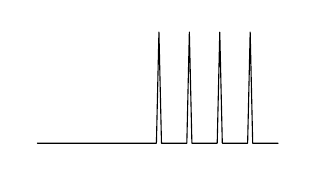
\begin{tikzpicture}[x=1pt,y=1pt]
\definecolor{fillColor}{RGB}{255,255,255}
\path[use as bounding box,fill=fillColor,fill opacity=0.00] (0,0) rectangle ( 93.95, 43.36);
\begin{scope}
\path[clip] (  0.00,  0.00) rectangle ( 93.95, 43.36);
\definecolor{drawColor}{RGB}{0,0,0}

\path[draw=drawColor,line width= 0.4pt,line join=round,line cap=round] (  3.48,  1.61) --
	(  4.40,  1.61) --
	(  5.31,  1.61) --
	(  6.23,  1.61) --
	(  7.14,  1.61) --
	(  8.06,  1.61) --
	(  8.97,  1.61) --
	(  9.89,  1.61) --
	( 10.81,  1.61) --
	( 11.72,  1.61) --
	( 12.64,  1.61) --
	( 13.55,  1.61) --
	( 14.47,  1.61) --
	( 15.38,  1.61) --
	( 16.30,  1.61) --
	( 17.22,  1.61) --
	( 18.13,  1.61) --
	( 19.05,  1.61) --
	( 19.96,  1.61) --
	( 20.88,  1.61) --
	( 21.79,  1.61) --
	( 22.71,  1.61) --
	( 23.63,  1.61) --
	( 24.54,  1.61) --
	( 25.46,  1.61) --
	( 26.37,  1.61) --
	( 27.29,  1.61) --
	( 28.20,  1.61) --
	( 29.12,  1.61) --
	( 30.04,  1.61) --
	( 30.95,  1.61) --
	( 31.87,  1.61) --
	( 32.78,  1.61) --
	( 33.70,  1.61) --
	( 34.61,  1.61) --
	( 35.53,  1.61) --
	( 36.44,  1.61) --
	( 37.36,  1.61) --
	( 38.28,  1.61) --
	( 39.19,  1.61) --
	( 40.11,  1.61) --
	( 41.02,  1.61) --
	( 41.94,  1.61) --
	( 42.85,  1.61) --
	( 43.77,  1.61) --
	( 44.69,  1.61) --
	( 45.60,  1.61) --
	( 46.52,  1.61) --
	( 47.43, 41.76) --
	( 48.35,  1.61) --
	( 49.26,  1.61) --
	( 50.18,  1.61) --
	( 51.10,  1.61) --
	( 52.01,  1.61) --
	( 52.93,  1.61) --
	( 53.84,  1.61) --
	( 54.76,  1.61) --
	( 55.67,  1.61) --
	( 56.59,  1.61) --
	( 57.51,  1.61) --
	( 58.42, 41.76) --
	( 59.34,  1.61) --
	( 60.25,  1.61) --
	( 61.17,  1.61) --
	( 62.08,  1.61) --
	( 63.00,  1.61) --
	( 63.92,  1.61) --
	( 64.83,  1.61) --
	( 65.75,  1.61) --
	( 66.66,  1.61) --
	( 67.58,  1.61) --
	( 68.49,  1.61) --
	( 69.41, 41.76) --
	( 70.33,  1.61) --
	( 71.24,  1.61) --
	( 72.16,  1.61) --
	( 73.07,  1.61) --
	( 73.99,  1.61) --
	( 74.90,  1.61) --
	( 75.82,  1.61) --
	( 76.74,  1.61) --
	( 77.65,  1.61) --
	( 78.57,  1.61) --
	( 79.48,  1.61) --
	( 80.40, 41.76) --
	( 81.31,  1.61) --
	( 82.23,  1.61) --
	( 83.15,  1.61) --
	( 84.06,  1.61) --
	( 84.98,  1.61) --
	( 85.89,  1.61) --
	( 86.81,  1.61) --
	( 87.72,  1.61) --
	( 88.64,  1.61) --
	( 89.56,  1.61) --
	( 90.47,  1.61);
\end{scope}
\end{tikzpicture}

\end{column}
\end{columns}

\begin{columns}
\begin{column}{0.6\textwidth}
\textbf{Transitory Change} (TC) 
\end{column}
\begin{column}{0.3\textwidth}
% Created by tikzDevice version 0.10.1 on 2017-12-13 18:19:58
% !TEX encoding = UTF-8 Unicode
\begin{tikzpicture}[x=1pt,y=1pt]
\definecolor{fillColor}{RGB}{255,255,255}
\path[use as bounding box,fill=fillColor,fill opacity=0.00] (0,0) rectangle ( 93.95, 43.36);
\begin{scope}
\path[clip] (  0.00,  0.00) rectangle ( 93.95, 43.36);
\definecolor{drawColor}{RGB}{0,0,0}

\path[draw=drawColor,line width= 0.4pt,line join=round,line cap=round] (  3.48,  1.61) --
	(  4.40,  1.61) --
	(  5.31,  1.61) --
	(  6.23,  1.61) --
	(  7.14,  1.61) --
	(  8.06,  1.61) --
	(  8.97,  1.61) --
	(  9.89,  1.61) --
	( 10.81,  1.61) --
	( 11.72,  1.61) --
	( 12.64,  1.61) --
	( 13.55,  1.61) --
	( 14.47,  1.61) --
	( 15.38,  1.61) --
	( 16.30,  1.61) --
	( 17.22,  1.61) --
	( 18.13,  1.61) --
	( 19.05,  1.61) --
	( 19.96,  1.61) --
	( 20.88,  1.61) --
	( 21.79,  1.61) --
	( 22.71,  1.61) --
	( 23.63,  1.61) --
	( 24.54,  1.61) --
	( 25.46,  1.61) --
	( 26.37,  1.61) --
	( 27.29,  1.61) --
	( 28.20,  1.61) --
	( 29.12,  1.61) --
	( 30.04,  1.61) --
	( 30.95,  1.61) --
	( 31.87,  1.61) --
	( 32.78,  1.61) --
	( 33.70,  1.61) --
	( 34.61,  1.61) --
	( 35.53,  1.61) --
	( 36.44,  1.61) --
	( 37.36,  1.61) --
	( 38.28,  1.61) --
	( 39.19,  1.61) --
	( 40.11,  1.61) --
	( 41.02,  1.61) --
	( 41.94,  1.61) --
	( 42.85,  1.61) --
	( 43.77,  1.61) --
	( 44.69,  1.61) --
	( 45.60,  1.61) --
	( 46.52,  1.61) --
	( 47.43, 41.76) --
	( 48.35, 29.71) --
	( 49.26, 21.28) --
	( 50.18, 15.38) --
	( 51.10, 11.25) --
	( 52.01,  8.35) --
	( 52.93,  6.33) --
	( 53.84,  4.91) --
	( 54.76,  3.92) --
	( 55.67,  3.23) --
	( 56.59,  2.74) --
	( 57.51,  2.40) --
	( 58.42,  2.16) --
	( 59.34,  2.00) --
	( 60.25,  1.88) --
	( 61.17,  1.80) --
	( 62.08,  1.74) --
	( 63.00,  1.70) --
	( 63.92,  1.67) --
	( 64.83,  1.65) --
	( 65.75,  1.64) --
	( 66.66,  1.63) --
	( 67.58,  1.62) --
	( 68.49,  1.62) --
	( 69.41,  1.61) --
	( 70.33,  1.61) --
	( 71.24,  1.61) --
	( 72.16,  1.61) --
	( 73.07,  1.61) --
	( 73.99,  1.61) --
	( 74.90,  1.61) --
	( 75.82,  1.61) --
	( 76.74,  1.61) --
	( 77.65,  1.61) --
	( 78.57,  1.61) --
	( 79.48,  1.61) --
	( 80.40,  1.61) --
	( 81.31,  1.61) --
	( 82.23,  1.61) --
	( 83.15,  1.61) --
	( 84.06,  1.61) --
	( 84.98,  1.61) --
	( 85.89,  1.61) --
	( 86.81,  1.61) --
	( 87.72,  1.61) --
	( 88.64,  1.61) --
	( 89.56,  1.61) --
	( 90.47,  1.61);
\end{scope}
\end{tikzpicture}

\end{column}
\end{columns}

\end{frame}

\subsection{Methodology of the study}\label{methodology-of-the-study-1}

\begin{frame}{Methodology used}

On European IPI: 1. \highlightbf{identification} and
\highlightbf{estimation} of the model over 12 years

\begin{enumerate}
\def\labelenumi{\arabic{enumi}.}
\setcounter{enumi}{1}
\item
  The raw series is corrected for outliers in the year of the
  introduction of the break and it is rebased to 100 at the month of the
  introduction of the break
\item
  simulation of a break, 5 years after the beginning of the time series
  date, of level 10 for a \highlightbf{additive} model
\item
  The regressor related to the simulated break is added to the Reg-ARIMA
  model and its coefficient it is estimated by freezing the estimates of
  all other parameters and \highlightbf{setting} the first estimated
  date
\end{enumerate}

We considered that the series has converged when:
\[\left\lvert\frac{\text{estimated value}}{\text{last estimated value}}-1\right\rvert < 5\;\%\]

\end{frame}

\subsection{Example}\label{example}

\begin{frame}{Example of a AO for IPI IT-1413 (manufacture of other
outerwear)}

\centering

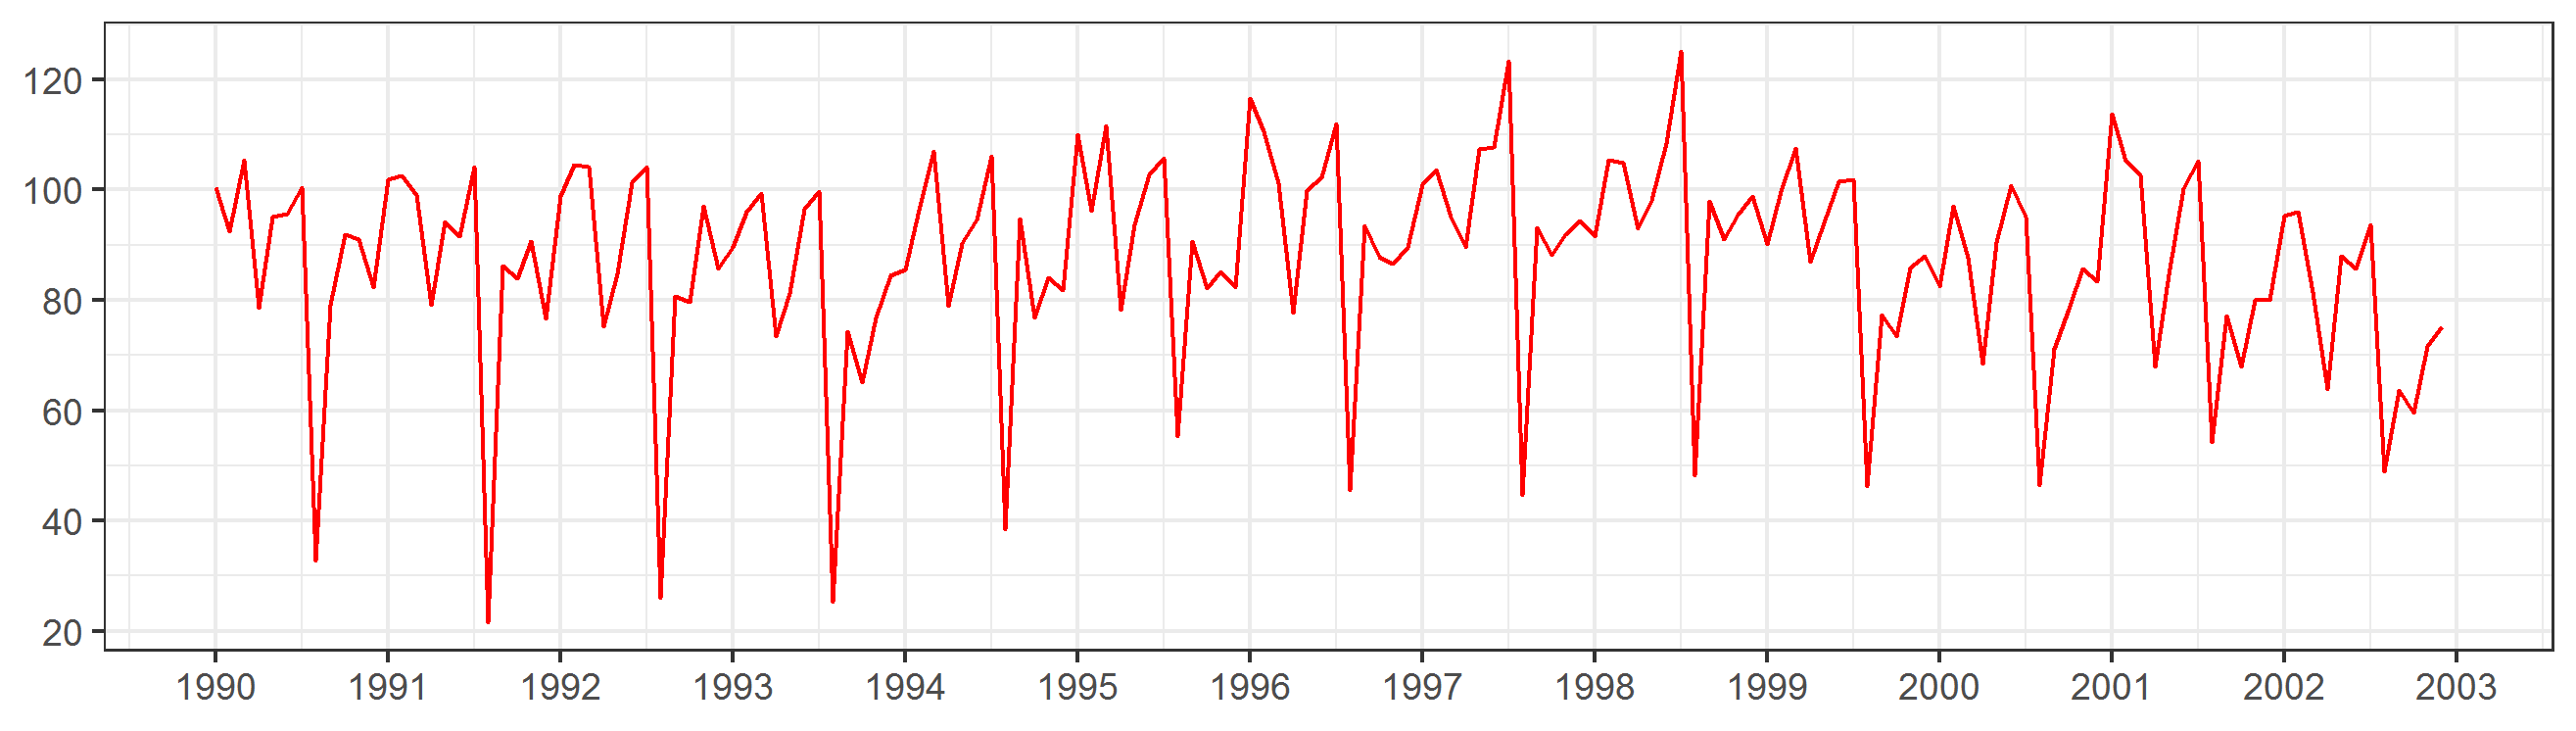
\includegraphics[width=0.95\textwidth]{img/AO_ipi_it1413_y.png}

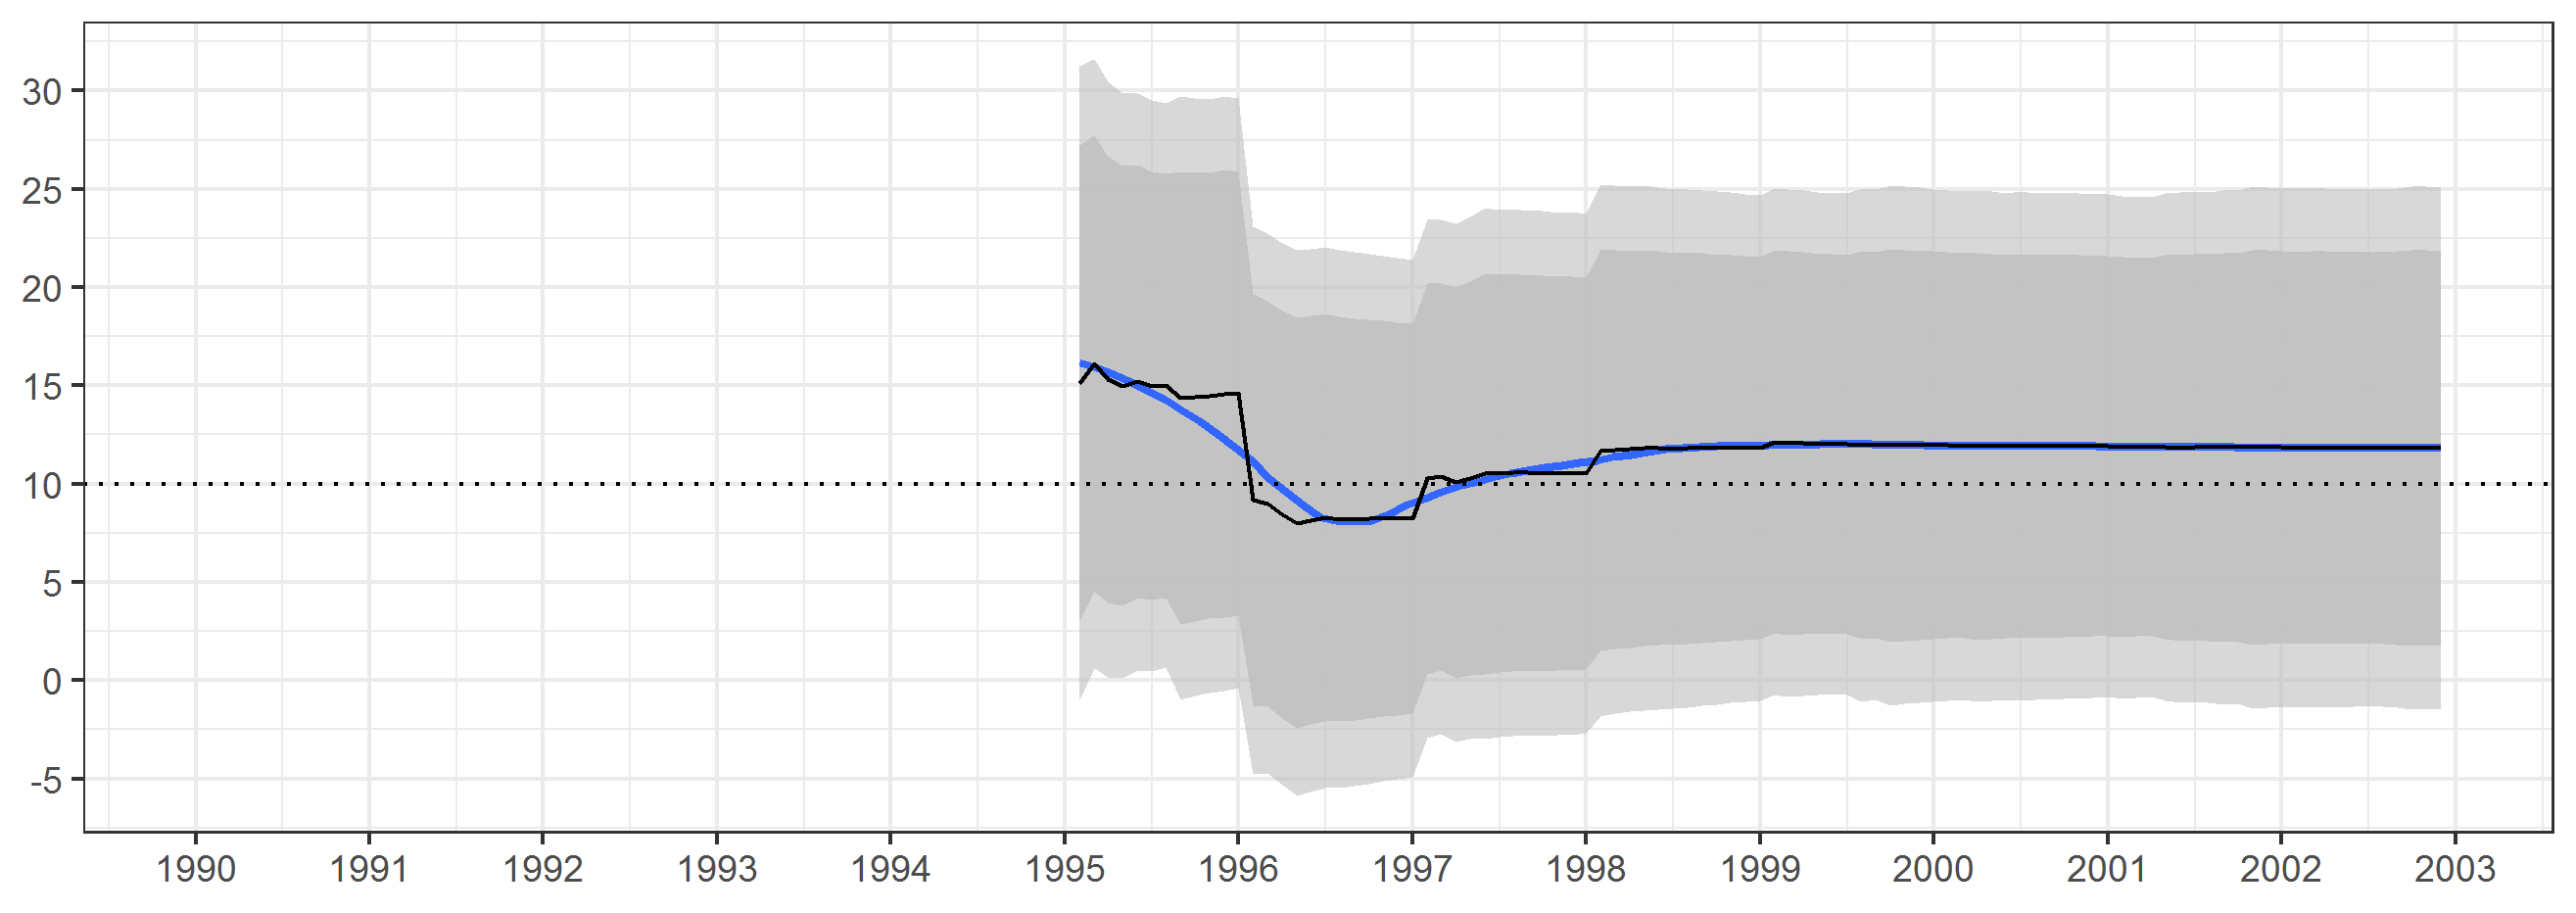
\includegraphics[width=0.95\textwidth]{img/AO_ipi_it1413_est.png}

\end{frame}

\subsection{Résultats des simulations}\label{resultats-des-simulations}

\begin{frame}{A rather slow convergence..}

\centering
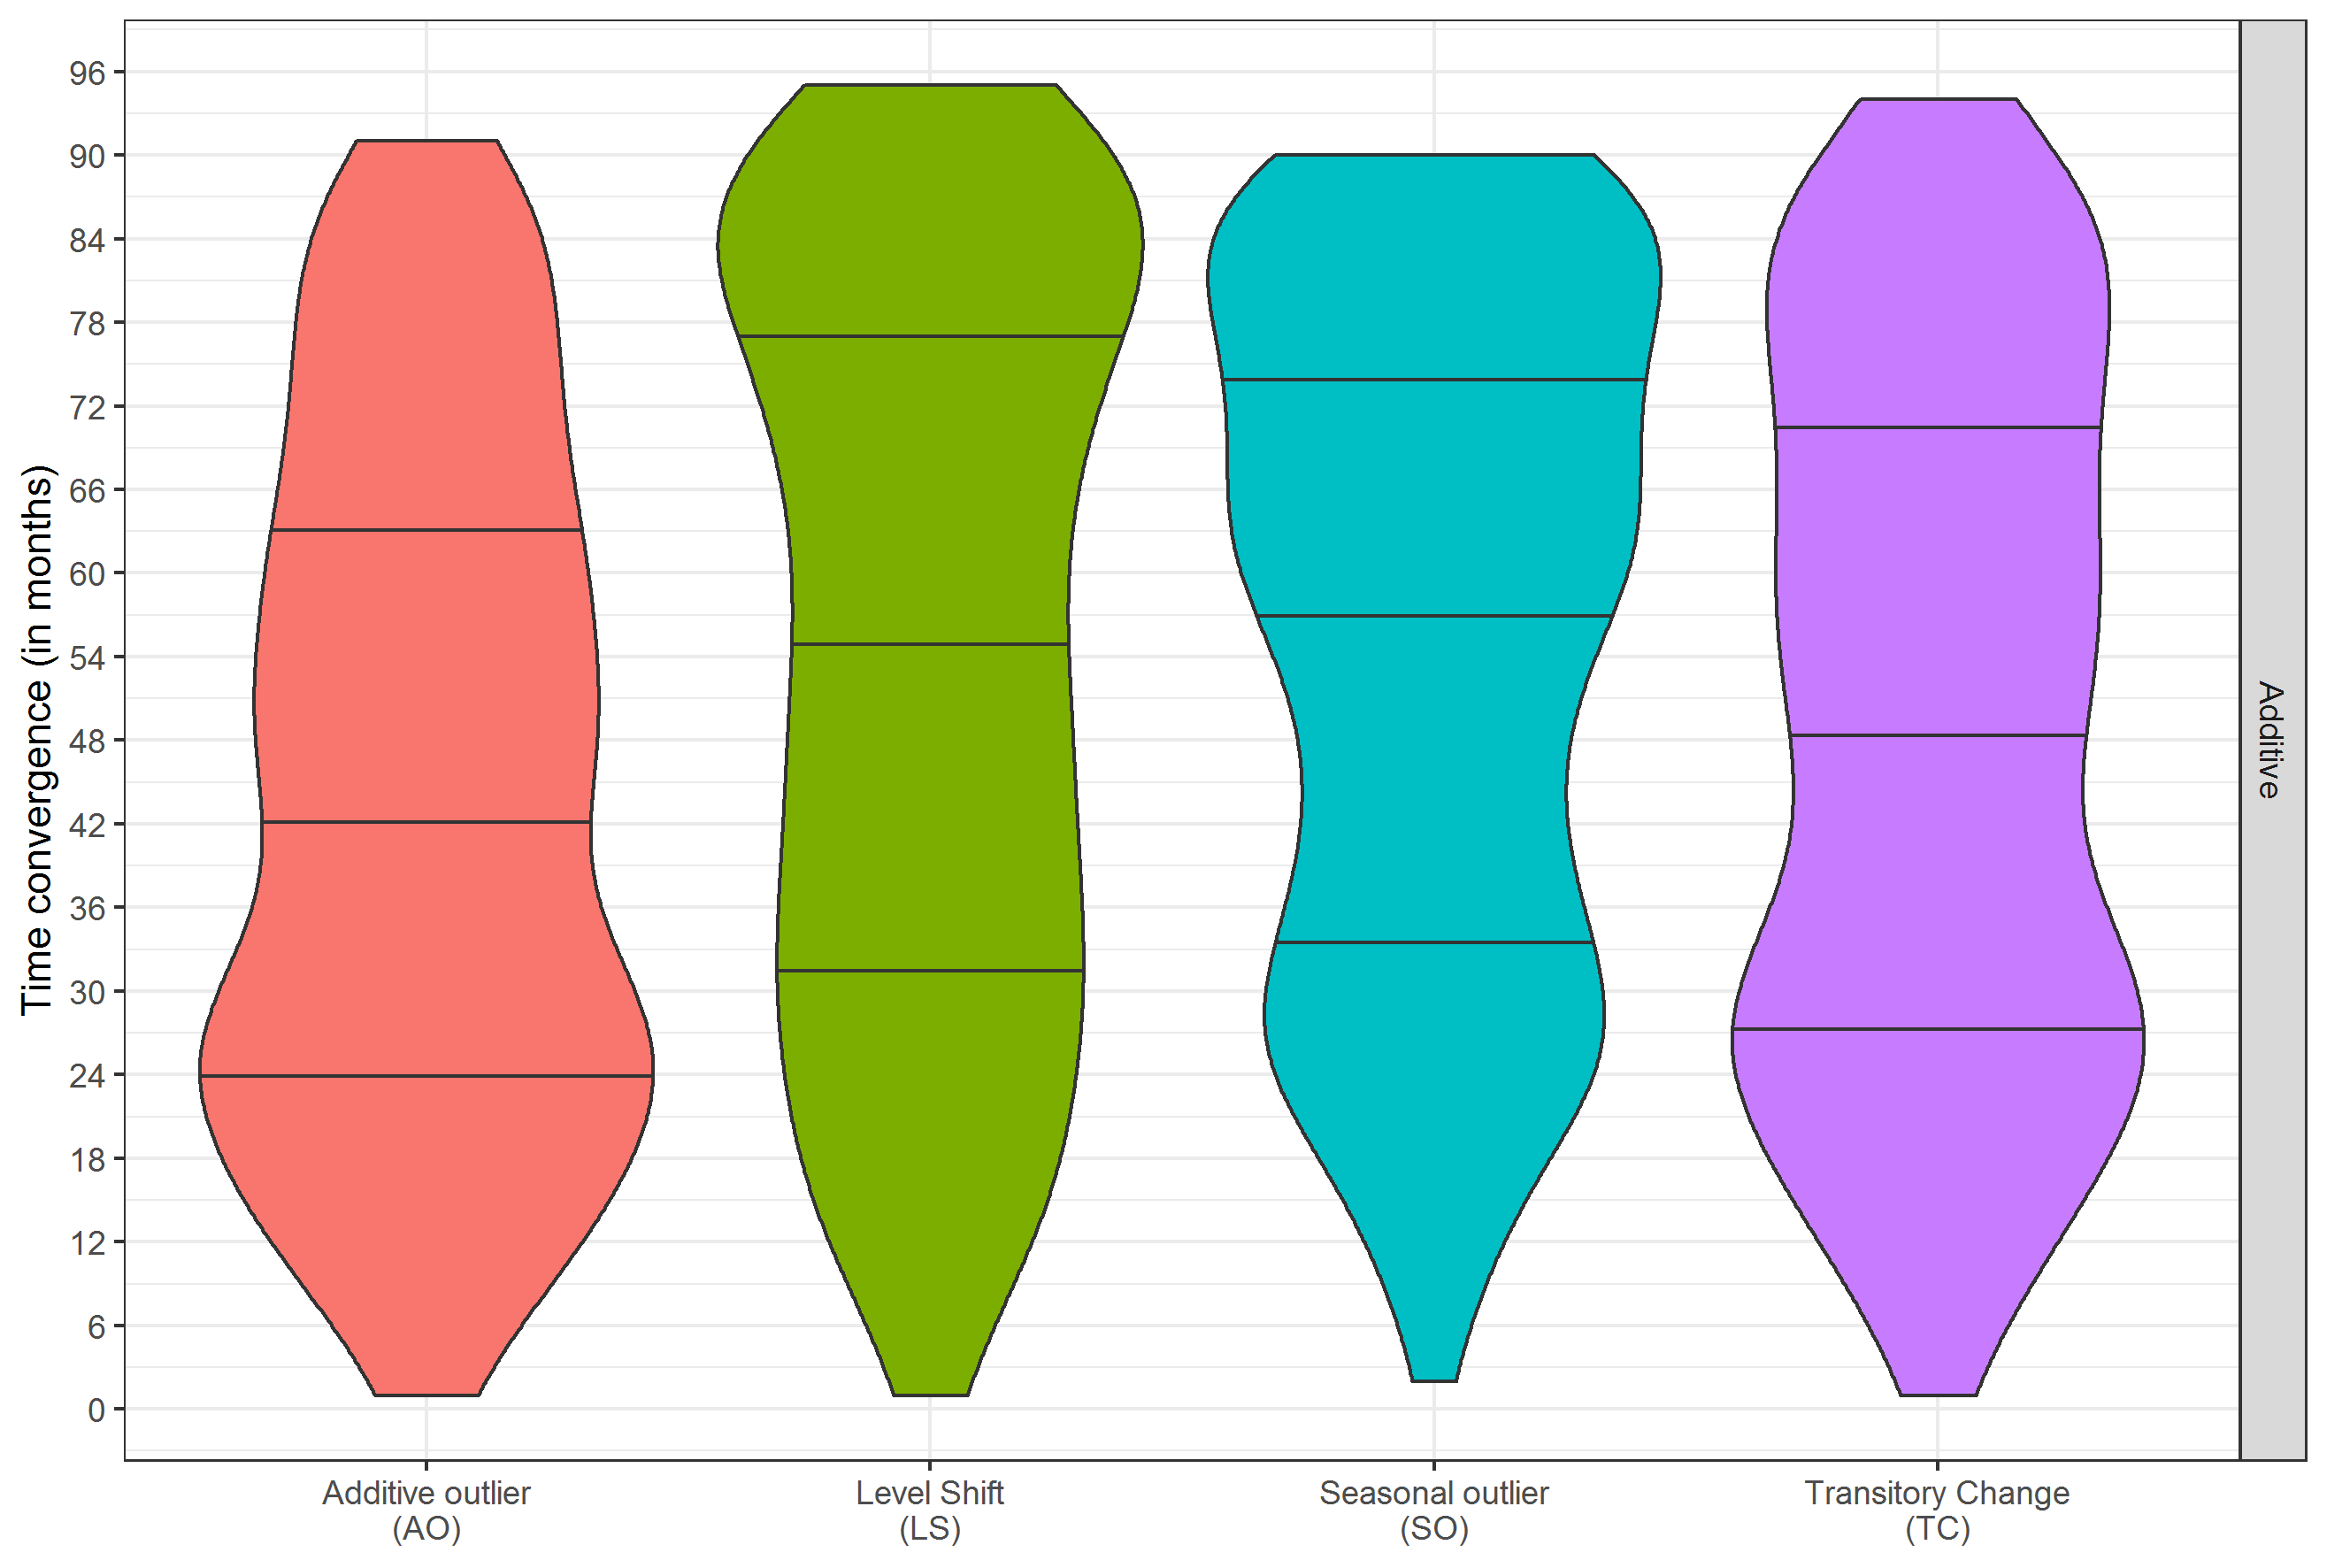
\includegraphics[width=1.00000\textwidth]{img/outliers_convergence_additif_5.png}\\

\end{frame}

\begin{frame}{\ldots{} But not always to the right value}

\centering

\begin{tabular}{lccccc}\toprule
  & Minimum & 25   \% & 50   \% & 75   \% & Maximum\\\midrule
\addlinespace[0.3em]\multicolumn{6}{l}{\textbf{Additive models}}\\
\hspace{1em}Additive outlier (AO) & -11.6 & 7.8 & 11.1 & 14.2 & 36.9\\
\hspace{1em}Level Shift (LS) & -11.4 & 5.6 & 9.3 & 12.7 & 49.8\\
\hspace{1em}Seasonal outlier (SO) & -5.8 & 7.3 & 8.8 & 11.0 & 31.1\\
\hspace{1em}Transitory Change (TC) & -17.4 & 6.5 & 10.2 & 14.1 & 47.2\\\addlinespace[0.3em]
\bottomrule\end{tabular}

\end{frame}

\section{Identification of the ARIMA
model}\label{identification-of-the-arima-model}

\begin{frame}{Identification of two equivalent models}

We use the same model in two different forms mathematically equivalent:

\begin{enumerate}
\def\labelenumi{\arabic{enumi}.}
\item
  The leap year regressor is added as a working days regressor
\item
  The leap year regressor is added as an external regressos
\end{enumerate}

\(\rightarrow\) study of the automatic models

\end{frame}

\begin{frame}{Different automatic models}

\centering
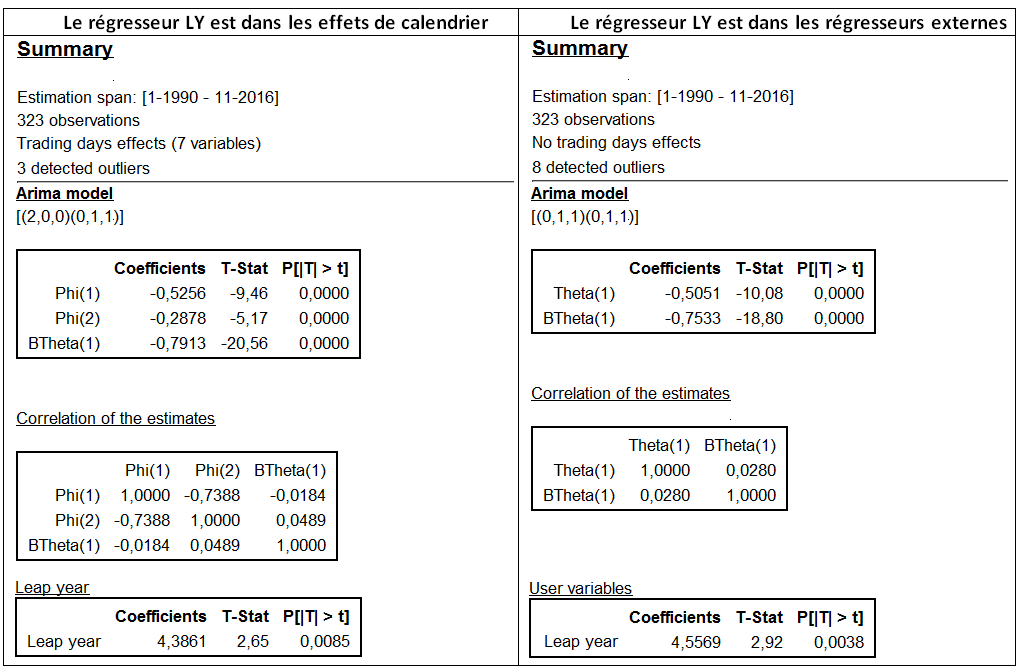
\includegraphics[width = \textwidth]{img/CholeskyRF241.png}

\end{frame}

\section{Conclusion and
recommendations}\label{conclusion-and-recommendations}

\begin{frame}{CConclusion and recommendations (1/2)}

\medskip

\bcinfo Simulations are \highlightbfslide{1}{questionables} and
\highlightbfslide{1}{can be improved} but highlight a
\highlightbfslide{1}{potential instability} of Reg-ARIMA models often
used as black boxes

\medskip  \pause
\bcsmbh Instabilities have a \highlightbfslide{2}{limited effect} on the
SA-WD series\dots \bcsmmh but have an impact on the
\highlightbfslide{2}{short term} history and on
\highlightbfslide{2}{revisions} !

\medskip  \pause
\bcattention Automatic algorithms use in X-13ARIMA-SEATS and TRAMO-SEATS
are \highlightbfslide{3}{important} and very
\highlightbfslide{3}{useful}

\end{frame}

\begin{frame}{Conclusion and recommendations (2/2)}

Specify the model \highlightbf{beforehand} at the level of the series
\highlightbf{series}:

\begin{itemize}
\item
  base selection procedures on economic reasoning (pay attention to long
  series)
\item
  \bcinterdit do not use methods like black boxes\ldots{}
  \pause Otherwise, you will be like this statistician who\ldots{}
\end{itemize}

\end{frame}

\begin{frame}{Thank you for your attention}

\begin{quote}
"He uses statistics as a drunk man uses lamp-posts: for support rather than for illumination.
\end{quote}

Quote widely attributed to Andrew Lang (1844-1912)

\addtocounter{framenumber}{-1}

\end{frame}

\end{document}
